% Provenance (never printed): cycle 3 "La planete Terre" and geography
% (weather and climate; reading a climate chart; the great climate zones of
% the world, hot, temperate and cold); see sources/book1/PROVENANCE.md.
% Book 1, grade 5, chapter 2.
\chapter{Weather and Climate}\label{ch:g5:weather-and-climate}

In the second week of January, two postcards arrive at the school. The
first one, from Lena's cousin, shows children building a \omterm{def:g3:stones-pebbles-sand:sand}{sand} castle on a
sunny beach under palm trees. The second one, from Tom's grandmother, shows
children building a snowman in a snowy garden. ``How can it be summer and
winter in the same week?'' asks Tom.

It is not the \omterm{def:g1:watching-the-weather:weather}{weather} of one day that differs so much between the two
places. It is the \omterm{def:g1:watching-the-weather:weather}{weather} they have, year after year: their \omterm{def:g5:weather-and-climate:climate}{climate}.

\begin{omfigure}
\begin{minipage}[b]{0.48\linewidth}\centering

\includegraphics[width=\linewidth]{images/book1/ai/g5-beach-postcard.jpg}
\end{minipage}\hfill
\begin{minipage}[b]{0.48\linewidth}\centering

\includegraphics[width=\linewidth]{images/book1/ai/g5-snowman-postcard.jpg}
\end{minipage}

{\small Two postcards from the same week of January: a sunny beach and a
snowy garden.}
\end{omfigure}

\begin{recall}
The \omterm{def:g1:watching-the-weather:weather}{weather} is the state of the air at a given place and time: sunny,
cloudy, rainy, snowy, windy (\cref{ch:g1:watching-the-weather}). A
thermometer measures the temperature of the air, in degrees Celsius; a
\omterm{def:g4:clouds-rain-snow:rain-gauge}{rain gauge} measures the \omterm{def:g4:clouds-rain-snow:precipitation}{rain}, in millimetres
(\cref{ch:g4:clouds-rain-snow}). The \omterm{def:g3:continents-and-oceans:equator}{equator} runs round the middle of the
\omterm{def:g3:continents-and-oceans:globe}{globe}, halfway between the \omterm{def:g3:continents-and-oceans:poles}{North Pole} and the \omterm{def:g3:continents-and-oceans:poles}{South Pole}
(\cref{ch:g3:continents-and-oceans}). The physics books showed that the
Earth turns round the Sun in one year, and that its seasons come from the
tilt of its axis: in summer, the Sun climbs higher in the sky and the days
are longer.
\end{recall}

\section{Weather is today, climate is the usual}

The \omterm{def:g1:watching-the-weather:weather}{weather} changes from day to day, and even from hour to hour. \omterm{def:g5:weather-and-climate:climate}{Climate}
is something else.

\begin{definition}[Climate]\label{def:g5:weather-and-climate:climate}
The \emph{climate}\index{climate} of a place is the \omterm{def:g1:watching-the-weather:weather}{weather} it usually
has, month by month, over many years: how warm or cold, how wet or dry
each season is. \omterm{def:g1:watching-the-weather:weather}{Weather} scientists work it out by averaging the
measurements of 30 years.
% ledger: wmo:normal-30yr
\end{definition}

``It is raining this morning'' is a sentence about the \omterm{def:g1:watching-the-weather:weather}{weather}. ``It \omterm{def:g4:clouds-rain-snow:precipitation}{rains}
a lot in autumn here'' is a sentence about the \omterm{def:g5:weather-and-climate:climate}{climate}. A single cold day
in summer does not change the \omterm{def:g5:weather-and-climate:climate}{climate}; it is just unusual \omterm{def:g1:watching-the-weather:weather}{weather}.

\omterm{def:g1:watching-the-weather:weather}{Weather} scientists of the whole world use the same rule: they average
30 years of measurements. The averages used today are those of the years
1991 to 2020.
% ledger: wmo:normal-30yr

\section{The climate chart}

To show the \omterm{def:g5:weather-and-climate:climate}{climate} of a place in one picture, we draw a chart.

\begin{definition}[Climate chart]\label{def:g5:weather-and-climate:climate-chart}
A \emph{climate chart}\index{climate chart} shows, for each month of the
year, the average temperature of a place (a curve) and the average amount
of \omterm{def:g4:clouds-rain-snow:precipitation}{rain} and \omterm{def:g4:clouds-rain-snow:precipitation}{snow} that falls there (bars, in millimetres of water).
\end{definition}

\begin{omfigure}
\begin{tikzpicture}
  \begin{axis}[name=pax, width=0.55\linewidth, height=5.6cm, ymin=0, ymax=400,
      axis y line*=right, axis x line=none, ybar, bar width=7pt,
      ytick={0,100,...,400}, ylabel={rain (mm)}, xmin=0.4, xmax=12.6,
      tick label style={font=\scriptsize}, label style={font=\scriptsize},
      ylabel style={blue!60!black}]
    \addplot[fill=blue!40, draw=blue!60!black]
      table[x=month, y=prcp_mm] {figdata/out/grade-5-climate_charts-seattle.dat};
  \end{axis}
  \begin{axis}[width=0.55\linewidth, height=5.6cm, ymin=-30, ymax=40,
      axis y line*=left, axis x line*=bottom, xmin=0.4, xmax=12.6,
      xtick={1,...,12}, xticklabels={J,F,M,A,M,J,J,A,S,O,N,D},
      ytick={-30,-20,...,40}, ylabel={temperature ($^\circ$C)},
      tick label style={font=\scriptsize}, label style={font=\scriptsize},
      ylabel style={red!70!black}]
    \addplot[red!70!black, thick, mark=*, mark size=1.3pt]
      table[x=month, y=tavg_C] {figdata/out/grade-5-climate_charts-seattle.dat};
    \draw[gray!60] (axis cs:0.4,0) -- (axis cs:12.6,0);
    \begin{scope}[every node/.style={circle, draw, fill=white, inner sep=0.8pt,
        font=\scriptsize\bfseries}]
      \node[text=red!70!black, draw=red!70!black] at (axis cs:5.5,27) {1};
      \node[text=blue!60!black, draw=blue!60!black] at (axis cs:7,-19) {2};
    \end{scope}
  \end{axis}
  \node[anchor=north west, font=\scriptsize, align=left, text width=4.2cm]
    at ($(pax.outer north east)+(0.3,-0.1)$) {%
    \textcolor{red!70!black}{\textbf{1} The red curve: the average temperature
    of each month, read on the left scale.}\par\smallskip
    \textcolor{blue!60!black}{\textbf{2} The blue bars: the average rain of each
    month, read on the right scale.}\par\smallskip
    \textbf{3} The letters under the chart: the months, January to
    December.};
\end{tikzpicture}

{\small The \omterm{def:g5:weather-and-climate:climate-chart}{climate chart} of Seattle, a city on the west \omterm{def:g1:landscapes-around-us:water}{coast} of the United
States. Averages of the years 1991 to 2020 (data: NOAA).}
% ledger: data:b1-noaa-normals
\end{omfigure}

\begin{method}[Reading a climate chart]\label{met:g5:weather-and-climate:reading}
\begin{enumerate}
  \item Find the warmest and the coldest month on the red curve, and read
        their temperatures on the left scale. Is the curve flat (the same
        temperature all year) or does it rise and fall (warm and cold
        seasons)? Does it go below 0~$^\circ$C (frost)?
  \item Find the wettest and the driest month among the blue bars, and read
        them on the right scale. Are the bars tall or short? Is there a dry
        season?
  \item Put it together in one sentence: ``hot and dry all year'', ``mild
        and wet, with a dry summer''{\ldots}
\end{enumerate}
\end{method}

\begin{example}[Seattle]\label{ex:g5:weather-and-climate:seattle}
In Seattle, the warmest month is August (about 20~$^\circ$C) and the
coldest is December (about 6~$^\circ$C): the curve rises and falls, but it
never goes below freezing. The tallest bar is November's (about 160~mm),
the shortest July's (about 15~mm). One sentence: mild winters, cool
summers, wet in autumn and winter, rather dry in summer. In a whole year
about 1\,000~millimetres of \omterm{def:g4:clouds-rain-snow:precipitation}{rain} fall: a metre of water.
% ledger: data:b1-noaa-normals
\end{example}

\section{Four climates}

Here are the \omterm{def:g5:weather-and-climate:climate-chart}{climate charts} of four towns of the United States, far apart
from each other: Phoenix, in the \omterm{def:g5:weather-and-climate:desert}{desert} of Arizona; Hilo, on the island of
Hawaii in the middle of the Pacific \omterm{def:g2:water-on-earth:ocean}{Ocean}; Seattle, on the west \omterm{def:g1:landscapes-around-us:water}{coast}; and
Utqia\.gvik, in the far north of Alaska, on the \omterm{def:g1:landscapes-around-us:water}{coast} of the Arctic \omterm{def:g2:water-on-earth:ocean}{Ocean}.
All four charts use the same scales, so we can compare them at a glance.

\begin{omfigure}
\def\gfivechart#1#2{%
\begin{tikzpicture}
  \begin{axis}[width=0.5\linewidth, height=4.6cm, ymin=0, ymax=400,
      axis y line*=right, axis x line=none, ybar, bar width=4pt,
      ytick={0,100,...,400}, xmin=0.4, xmax=12.6,
      tick label style={font=\tiny}]
    \addplot[fill=blue!40, draw=blue!60!black]
      table[x=month, y=prcp_mm] {figdata/out/grade-5-climate_charts-#1.dat};
  \end{axis}
  \begin{axis}[width=0.5\linewidth, height=4.6cm, ymin=-30, ymax=40,
      axis y line*=left, axis x line*=bottom, xmin=0.4, xmax=12.6,
      xtick={1,...,12}, xticklabels={J,F,M,A,M,J,J,A,S,O,N,D},
      ytick={-30,-20,...,40}, tick label style={font=\tiny},
      title={#2}, title style={font=\scriptsize\bfseries, yshift=-4pt}]
    \addplot[red!70!black, thick, mark=*, mark size=1pt]
      table[x=month, y=tavg_C] {figdata/out/grade-5-climate_charts-#1.dat};
    \draw[gray!60] (axis cs:0.4,0) -- (axis cs:12.6,0);
  \end{axis}
\end{tikzpicture}}%
\gfivechart{phoenix}{Phoenix: a hot \omterm{def:g5:weather-and-climate:desert}{desert}}\hfill
\gfivechart{hilo}{Hilo: a \omterm{def:g5:weather-and-climate:rainforest}{rainforest} \omterm{def:g5:weather-and-climate:climate}{climate}}

\medskip
\gfivechart{seattle}{Seattle: a temperate \omterm{def:g5:weather-and-climate:climate}{climate}}\hfill
\gfivechart{utqiagvik}{Utqia\.gvik: a polar \omterm{def:g5:weather-and-climate:climate}{climate}}

{\small Four \omterm{def:g5:weather-and-climate:climate-chart}{climate charts} with the same scales: temperature in
$^\circ$C on the left (red curve), \omterm{def:g4:clouds-rain-snow:precipitation}{rain} in millimetres on the right (blue
bars). Averages of the years 1991 to 2020 (data: NOAA).}
% ledger: data:b1-noaa-normals
\end{omfigure}

\paragraph{The desert.} In Phoenix, the bars are so short that we can
hardly see them: in a whole year, less than 200 millimetres of \omterm{def:g4:clouds-rain-snow:precipitation}{rain} fall.
The summers are very hot: in July the average temperature is 35 degrees.
% ledger: data:b1-noaa-normals

\begin{definition}[Desert]\label{def:g5:weather-and-climate:desert}
A \emph{desert}\index{desert} is a place where very little \omterm{def:g4:clouds-rain-snow:precipitation}{rain} falls:
less than 250 millimetres in a year. Few plants can live there, and the
ground is often bare.
% ledger: usgs:arid-250mm
\end{definition}

\omterm{def:g5:weather-and-climate:desert}{Deserts} are not always hot. Look at Utqia\.gvik: less than 150 millimetres
fall there in a year, even less than in Phoenix: it is a cold \omterm{def:g5:weather-and-climate:desert}{desert}.
\omterm{def:g5:weather-and-climate:desert}{Deserts} can be hot or cold.
% ledger: data:b1-noaa-normals, usgs:arid-250mm

\paragraph{The rainforest.} Hilo is the opposite of Phoenix. Its bars are
the tallest of the four charts: more than 3\,000 millimetres of \omterm{def:g4:clouds-rain-snow:precipitation}{rain} fall in
a year, and every month is wet. And its red curve is almost flat: between
22 and 25 degrees all year. There is no winter at all.
% ledger: data:b1-noaa-normals

\begin{definition}[Rainforest]\label{def:g5:weather-and-climate:rainforest}
A \emph{rainforest}\index{rainforest} is a thick forest of very tall trees
that grows where it is warm and wet all year round, with heavy \omterm{def:g4:clouds-rain-snow:precipitation}{rain} in
every month. Most rainforests lie near the \omterm{def:g3:continents-and-oceans:equator}{equator}.
\end{definition}

\begin{omfigure}
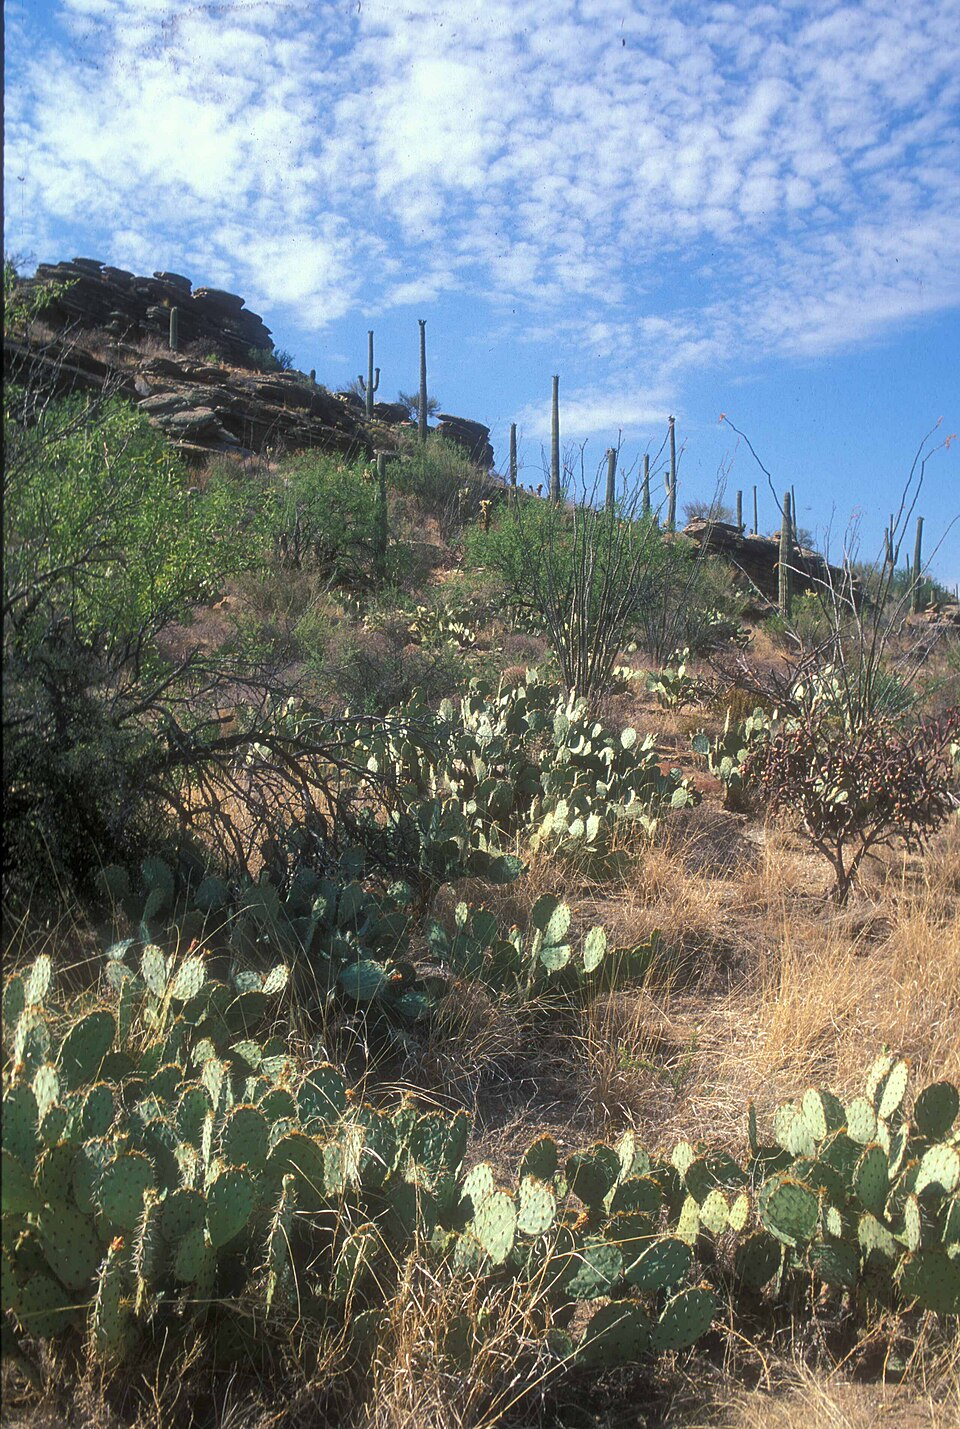
\includegraphics[height=3.6cm]{images/book1/g5-sonoran-desert.jpg}\quad
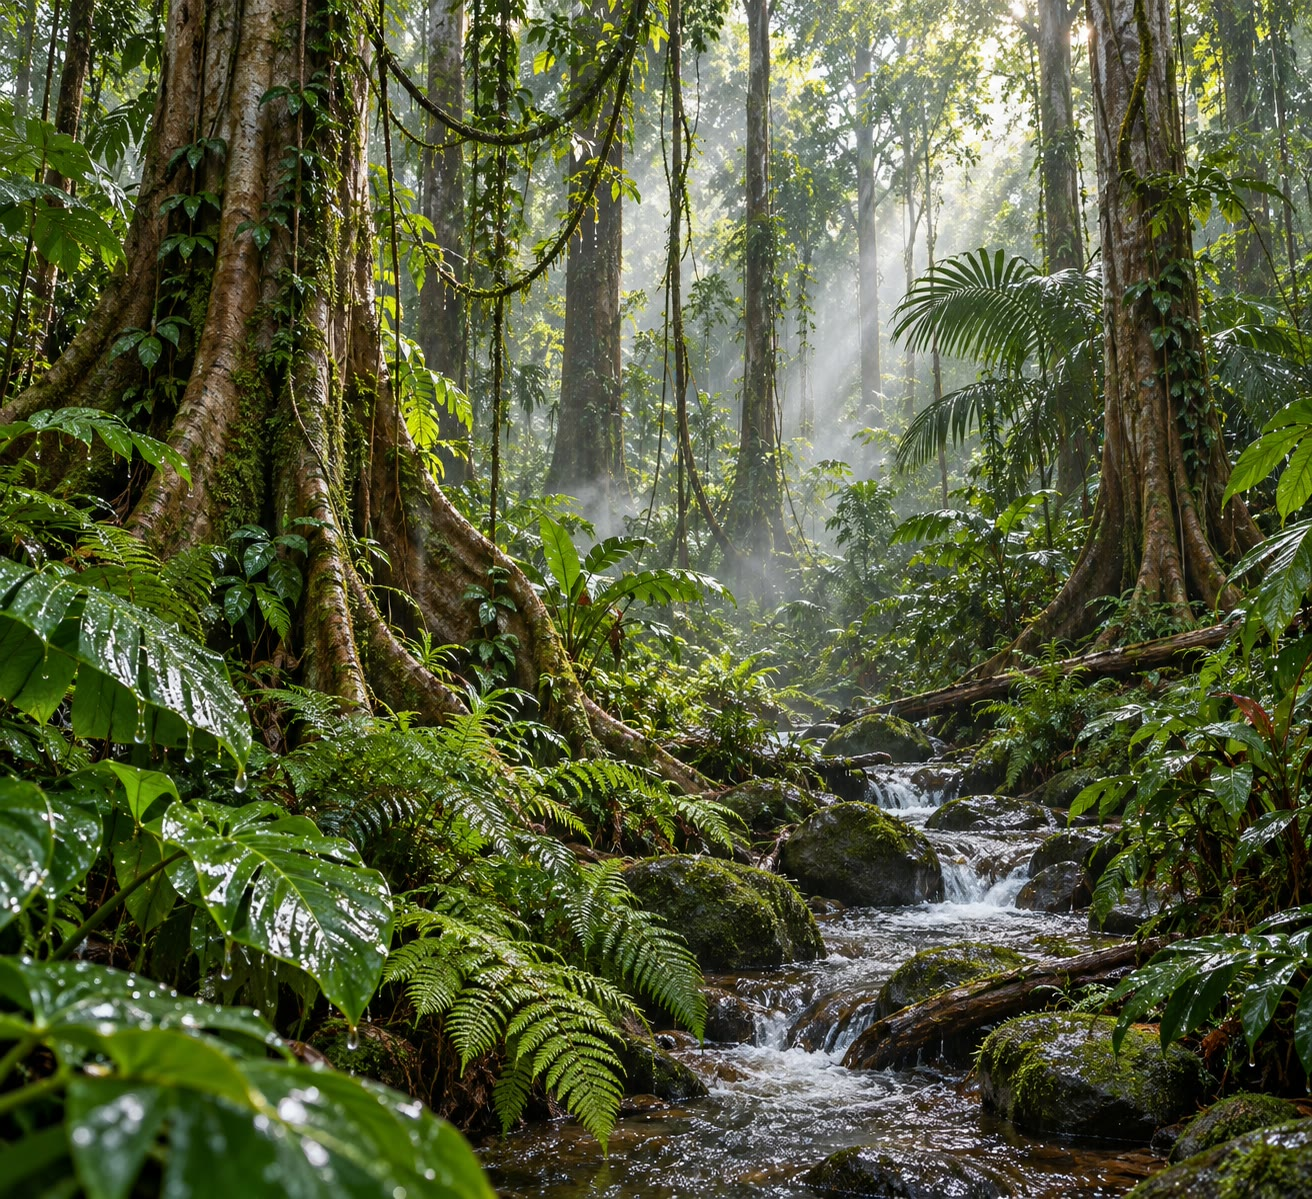
\includegraphics[height=3.6cm]{images/book1/ai/g5-rainforest.jpg}\quad
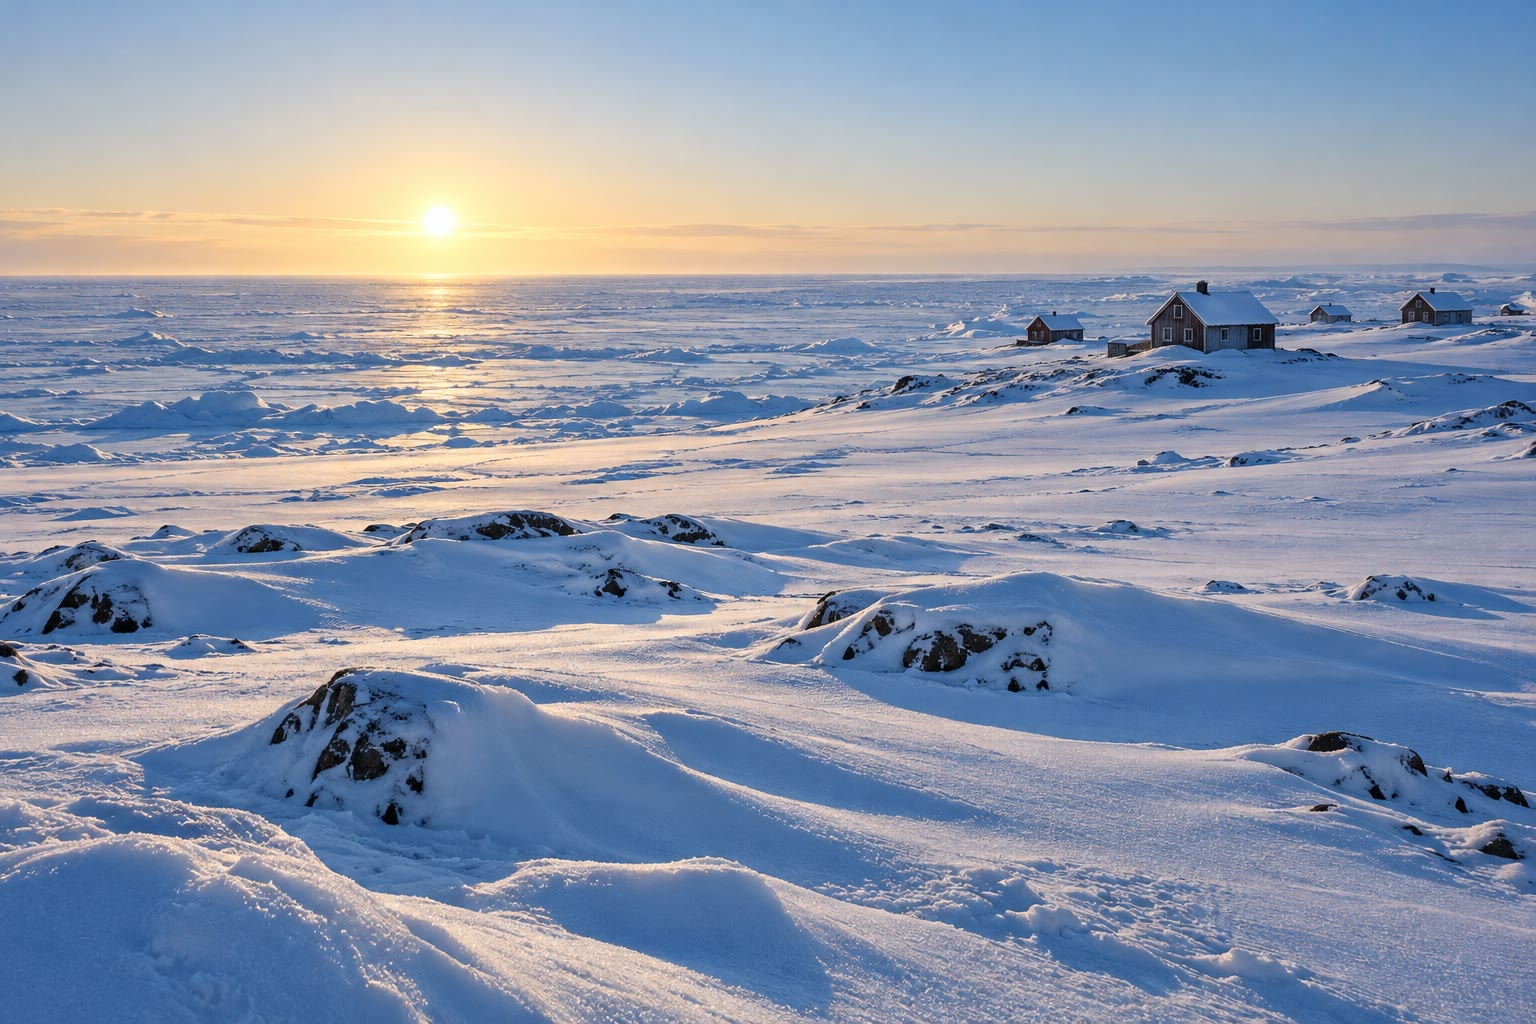
\includegraphics[height=3.6cm]{images/book1/ai/g5-polar-tundra.jpg}

{\small Three extreme \omterm{def:g5:weather-and-climate:climate}{climates}. Left: the Sonoran \omterm{def:g5:weather-and-climate:desert}{Desert} in Arizona, the
\omterm{def:g5:weather-and-climate:desert}{desert} of Phoenix, with tall saguaro cacti and prickly pears, which store
water in their thick stems (photograph: U.S. National Park Service, Saguaro
National Park, public domain). Middle: inside a \omterm{def:g5:weather-and-climate:rainforest}{rainforest} after a shower.
Right: a polar \omterm{def:g1:landscapes-around-us:water}{coast} in winter, with a frozen \omterm{def:g2:water-on-earth:ocean}{sea} and a low Sun at midday.}
% ledger: nps:sonoran-desert
\end{omfigure}

\paragraph{The temperate climate.} Seattle is in between: its curve rises
in summer and falls in winter, but never very far; it \omterm{def:g4:clouds-rain-snow:precipitation}{rains} a fair amount,
mostly in autumn and winter. This is a temperate \omterm{def:g5:weather-and-climate:climate}{climate}: no great heat,
no great cold.

\paragraph{The polar climate.} In Utqia\.gvik, the red curve stays below
0~$^\circ$C for eight months of the year; in February the average is
24 degrees below zero. Even in July, the warmest month, it is only about
5 degrees.
% ledger: data:b1-noaa-normals

\section{Hot, temperate and cold zones}

Why is it warm near the \omterm{def:g3:continents-and-oceans:equator}{equator} and cold near the \omterm{def:g3:continents-and-oceans:poles}{poles}? Because of the
Sun. Near the \omterm{def:g3:continents-and-oceans:equator}{equator}, the midday Sun stands high in the sky all year
round: its light falls almost straight down and warms the ground strongly.
Near the \omterm{def:g3:continents-and-oceans:poles}{poles}, the Sun always stays low: its light arrives slanting,
spread over a large area, and it warms little. In winter there, the Sun
may not rise at all.

Two pairs of lines around the \omterm{def:g3:continents-and-oceans:globe}{globe} divide the Earth into \omterm{def:g5:weather-and-climate:climate-zone}{climate zones}.

\begin{definition}[Tropics and polar circles]\label{def:g5:weather-and-climate:tropics}
The two \emph{tropics}\index{tropic} are the lines around the \omterm{def:g3:continents-and-oceans:globe}{globe}, one north
and one south of the \omterm{def:g3:continents-and-oceans:equator}{equator}, that mark how far from the \omterm{def:g3:continents-and-oceans:equator}{equator} the
midday Sun can be straight overhead: the Tropic of Cancer in the north,
the Tropic of Capricorn in the south. The two \emph{polar
circles}\index{polar circle} are the lines around the \omterm{def:g3:continents-and-oceans:globe}{globe}, near the
\omterm{def:g3:continents-and-oceans:poles}{poles}, beyond which, in the middle of winter, the Sun does not rise for at
least one day, and in the middle of summer it does not set: the Arctic
Circle in the north, the Antarctic Circle in the south.
\end{definition}

The tilt of the Earth's axis decides where these lines lie.

\begin{definition}[Climate zones]\label{def:g5:weather-and-climate:climate-zone}
The Earth is divided into three kinds of \emph{climate zone}\index{climate
zone}: the \emph{hot zone}, between the two \omterm{def:g5:weather-and-climate:tropics}{tropics}, around the \omterm{def:g3:continents-and-oceans:equator}{equator};
the two \emph{temperate zones}, between a \omterm{def:g5:weather-and-climate:tropics}{tropic} and a \omterm{def:g5:weather-and-climate:tropics}{polar circle}, where
summers and winters differ; and the two \emph{cold zones}, beyond the
\omterm{def:g5:weather-and-climate:tropics}{polar circles}, around the \omterm{def:g3:continents-and-oceans:poles}{poles}.
\end{definition}

\begin{omfigure}
\begin{tikzpicture}
\begin{axis}[ommap, width=\linewidth, xtick=\empty, ytick=\empty, grid=none,
    axis background/.style={fill=white}, clip=true]
  \addplot[fill=orange!35, draw=none] table {figdata/out/grade-5-climate_zones-hot.dat};
  \addplot[fill=green!20, draw=none] table {figdata/out/grade-5-climate_zones-temperate.dat};
  \addplot[fill=cyan!20, draw=none] table {figdata/out/grade-5-climate_zones-cold.dat};
  \addplot[fill=black!25, fill opacity=0.8, draw=black!60, line width=0.2pt]
    table {figdata/out/shared-geo-land.dat};
  \addplot[black!70, dashed, line width=0.5pt] table {figdata/out/grade-5-climate_zones-lines.dat};
  \draw[black!70, line width=0.6pt] (axis cs:-180,0) -- (axis cs:180,0);
  \addplot[only marks, mark=*, mark size=1.8pt, red!80!black]
    table[x=lon, y=lat] {figdata/out/grade-5-climate_zones-stations.dat};
  \begin{scope}[every node/.style={font=\scriptsize, fill=white, fill opacity=0.75,
      text opacity=1, inner sep=1pt}]
    \node[anchor=west] at (axis cs:-107,33.4) {Phoenix};
    \node[anchor=east] at (axis cs:-158,19.7) {Hilo};
    \node[anchor=west] at (axis cs:-117,47.4) {Seattle};
    \node[anchor=west] at (axis cs:-151,73.5) {Utqia\.gvik};
  \end{scope}
  \begin{scope}[every node/.style={font=\scriptsize\bfseries, align=center,
      fill=white, fill opacity=0.7, text opacity=1, inner sep=1pt}]
    \node at (axis cs:-5,83) {cold zone};
    \node at (axis cs:-40,40) {temperate zone};
    \node at (axis cs:-25,-8) {hot zone};
    \node at (axis cs:95,-45) {temperate zone};
    \node at (axis cs:-60,-80) {cold zone};
  \end{scope}
\end{axis}
\end{tikzpicture}

{\small The \omterm{def:g5:weather-and-climate:climate-zone}{climate zones}. From top to bottom, the dashed lines are the
Arctic Circle, the \omterm{def:g5:weather-and-climate:tropics}{Tropic} of Cancer, the \omterm{def:g5:weather-and-climate:tropics}{Tropic} of Capricorn and the
Antarctic Circle; the solid line is the \omterm{def:g3:continents-and-oceans:equator}{equator}. The red dots are the four
towns of the \omterm{def:g5:weather-and-climate:climate-chart}{climate charts} above.}
% ledger: earth:obliquity, data:b1-noaa-normals
\end{omfigure}

The zones give a first, rough picture. Inside each one, many other things
change the \omterm{def:g5:weather-and-climate:climate}{climate}: how far a place is from the \omterm{def:g2:water-on-earth:ocean}{sea}, how high it is, where
its winds come from. You will meet them in the later grades.

\begin{remark}[Phoenix and the zones]\label{rem:g5:weather-and-climate:phoenix}
On the \omterm{def:g2:drawing-to-map:map}{map} of the zones, Phoenix lies a little north of the \omterm{def:g5:weather-and-climate:tropics}{Tropic} of
Cancer, in the temperate zone, and yet it is a hot \omterm{def:g5:weather-and-climate:desert}{desert}. The zones are a
first, rough picture: many of the great hot \omterm{def:g5:weather-and-climate:desert}{deserts} lie near the \omterm{def:g5:weather-and-climate:tropics}{tropics},
on the edge of the hot zone, and you will learn why in
\cref{ch:g8:winds-global-circulation}.
\end{remark}

\section{Exercises}

\begin{exercise}[$\star$]\label{exo:g5:weather-and-climate:1}
\omterm{def:g1:watching-the-weather:weather}{Weather} or \omterm{def:g5:weather-and-climate:climate}{climate}?
\begin{enumerate}
  \item[(a)] It is snowing in Utqia\.gvik this morning.
  \item[(b)] In Phoenix, summers are very hot and dry.
  \item[(c)] Yesterday afternoon a strong wind blew in Seattle.
  \item[(d)] In Hilo, it \omterm{def:g4:clouds-rain-snow:precipitation}{rains} a lot in every month of the year.
\end{enumerate}
\end{exercise}

\begin{exercise}[$\star$]\label{exo:g5:weather-and-climate:2}
What is the \omterm{def:g5:weather-and-climate:climate}{climate} of a place? Over how many years do \omterm{def:g1:watching-the-weather:weather}{weather} scientists
average their measurements to describe it?
\end{exercise}

\begin{exercise}[$\star$]\label{exo:g5:weather-and-climate:3}
On the \omterm{def:g5:weather-and-climate:climate-chart}{climate chart} of Seattle, which is the coldest month? Which is the
wettest month? Does the temperature ever go below 0~$^\circ$C?
\end{exercise}

\begin{exercise}[$\star$]\label{exo:g5:weather-and-climate:4}
On the \omterm{def:g5:weather-and-climate:climate-chart}{climate chart} of Utqia\.gvik, which is the warmest month? Is any
month warmer than 10~$^\circ$C?
\end{exercise}

\begin{exercise}[$\star$]\label{exo:g5:weather-and-climate:5}
In which \omterm{def:g5:weather-and-climate:climate-zone}{climate zone} is each of these places: the \omterm{def:g3:continents-and-oceans:equator}{equator}; the \omterm{def:g3:continents-and-oceans:poles}{North
Pole}; a place halfway between the \omterm{def:g3:continents-and-oceans:equator}{equator} and the \omterm{def:g3:continents-and-oceans:poles}{South Pole}?
\end{exercise}

\begin{exercise}[$\star$]\label{exo:g5:weather-and-climate:6}
Use the \omterm{def:g2:drawing-to-map:map}{map} of the zones. In which \omterm{def:g5:weather-and-climate:climate-zone}{climate zone} is each of the four towns:
Phoenix, Hilo, Seattle, Utqia\.gvik?
\end{exercise}

\begin{exercise}[$\star\star$]\label{exo:g5:weather-and-climate:7}
Here is the average \omterm{def:g4:clouds-rain-snow:precipitation}{rain} of each month in Seattle, in millimetres, rounded
to whole numbers:
\begin{center}
\begin{tabular}{|*{12}{c|}}
\hline
J & F & M & A & M & J & J & A & S & O & N & D\\
\hline
147 & 96 & 106 & 81 & 48 & 37 & 15 & 25 & 41 & 99 & 160 & 145\\
\hline
\end{tabular}
\end{center}
How much \omterm{def:g4:clouds-rain-snow:precipitation}{rain} falls in Seattle in a whole year? How much falls in the
three months of December, January and February?
% ledger: data:b1-noaa-normals
\end{exercise}

\begin{exercise}[$\star\star$]\label{exo:g5:weather-and-climate:8}
In Phoenix, the average temperature is 14~$^\circ$C in January and
35~$^\circ$C in July. In Hilo, it is 22~$^\circ$C in January and
25~$^\circ$C in July. Compute the difference between July and January in
each town. Where do the seasons change the temperature more?
% ledger: data:b1-noaa-normals
\end{exercise}

\begin{exercise}[$\star\star$]\label{exo:g5:weather-and-climate:9}
Here are the averages of an imaginary town.
\begin{center}
\begin{tabular}{|l|*{12}{c|}}
\hline
month & J & F & M & A & M & J & J & A & S & O & N & D\\
\hline
temperature ($^\circ$C) & 27 & 27 & 28 & 28 & 28 & 27 & 27 & 27 & 27 & 27 & 27 & 27\\
\hline
\omterm{def:g4:clouds-rain-snow:precipitation}{rain} (mm) & 250 & 230 & 280 & 290 & 260 & 180 & 170 & 160 & 190 & 230 & 250 & 260\\
\hline
\end{tabular}
\end{center}
Is it a \omterm{def:g5:weather-and-climate:desert}{desert}, a \omterm{def:g5:weather-and-climate:rainforest}{rainforest}, a temperate or a polar \omterm{def:g5:weather-and-climate:climate}{climate}? Give two
reasons. In which zone is the town most likely to be?
\end{exercise}

\begin{exercise}[$\star\star$]\label{exo:g5:weather-and-climate:10}
Go back to the two postcards at the start of the chapter, sent in the same
week of January. Give two different explanations of how children can play
on a sunny beach in one place while others build a snowman in another.
\end{exercise}

\begin{exercise}[$\star\star\star$]\label{exo:g5:weather-and-climate:11}
Noor says: ``Phoenix and Seattle are both in the temperate zone, so they
must have the same \omterm{def:g5:weather-and-climate:climate}{climate}.'' Use the \omterm{def:g5:weather-and-climate:climate-chart}{climate charts} to show that she is
wrong: compare their temperatures and their \omterm{def:g4:clouds-rain-snow:precipitation}{rain}. Then say what the \omterm{def:g5:weather-and-climate:climate-zone}{climate
zones} tell us, and what they do not.
\end{exercise}
